The given lines can be represented in vector form as
\begin{align}\label{vec/2008/23/eq:1}
    \myvec{1&3}\vec{x}&=6 \\
    \label{vec/2008/23/eq:2}
        \myvec{2&-3}\vec{x}&=12
\end{align}
and 
the equation of y axis is
\begin{align}\label{vec/2008/23/eq:3}
    \myvec{1&0}\vec{x}=0
\end{align}

\begin{enumerate}
    \item Let line \eqref{vec/2008/23/eq:1} and line \eqref{vec/2008/23/eq:2} meet at point $\vec{P}$. Then,
    \begin{align}
        \myvec{1 & 3 \\ 2 & -3}\vec{P}&=
    \myvec{6 \\ 12}\\
\implies     \vec{P}&=\myvec{1 & 3 \\ 2 & -3}^{-1}\myvec{6 \\ 12}\\
&=\myvec{6\\0}
    \end{align}
    
    \item Let line \eqref{vec/2008/23/eq:1} and line \eqref{vec/2008/23/eq:3} meet at point $\vec{Q}$. Then,
    \begin{align}
        \myvec{1 & 3 \\ 1 & 0}\vec{Q}&=
    \myvec{6 \\ 0}\\
    \implies \vec{Q}&=\myvec{1 & 3 \\ 1 & 0}^{-1}\myvec{6 \\ 0}\\
    &=\myvec{0\\2}
    \end{align}
    
\item Let line \eqref{vec/2008/23/eq:2} and line \eqref{vec/2008/23/eq:3} meet at point $\vec{R}$. Then,
\begin{align}
    \myvec{2 & -3 \\ 1 & 0}\vec{R}&=
\myvec{12 \\ 0}\\
\implies \vec{R} &=\myvec{2 & -3 \\ 1 & 0}^{-1}\myvec{12 \\ 0}\\
&=\myvec{0\\-4}
\end{align}
\end{enumerate}
So $\triangle PQR$ is formed by intersection of \eqref{vec/2008/23/eq:1},
\eqref{vec/2008/23/eq:2} and \eqref{vec/2008/23/eq:3}.  See Fig.     \ref{vec/2008/23/Graphical solution}.
%
\begin{figure}[ht]
    \centering
    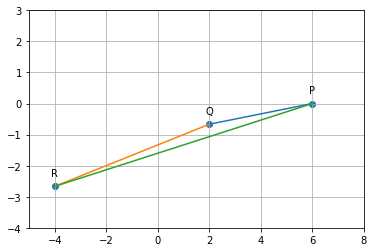
\includegraphics[width=\columnwidth]{vectors/solutions/2008/23/download.png}
    \caption{Graphical solution}
    \label{vec/2008/23/Graphical solution}
\end{figure}


